\documentclass[journal]{IEEEtran}
\usepackage{amsmath,amssymb,booktabs,graphicx,url,multirow,array}
\usepackage[hidelinks]{hyperref}

\begin{document}

\title{Drift-Aware Federated Human Activity Recognition:\\ Detection, Mode Typing and Cheap Local Adaptation on PAMAP2}

\author{\IEEEauthorblockN{Author names withheld for the draft}%
\thanks{Draft generated from the pre-registered experiments in this repository (\texttt{docs/analysis\_plan.md}, amendments A1--A5). Not yet reviewed by the authors.}}

\maketitle

\begin{abstract}
Wearable activity-recognition models deployed through federated learning (FL) degrade when sensor placement, gain or user behaviour changes after deployment. We study a client-side pipeline that detects drift from the model's own error stream, classifies whether the drift is \emph{virtual} (inputs change) or \emph{real} (labels change), and answers with a cheap response chosen by that type: a closed-form, label-conditioned input recalibration for virtual drift and continual head retraining with replay for real drift, neither of which uses uplink bandwidth. We build a ground-truth drift benchmark on PAMAP2 (8 clients, 12 classes, sudden, gradual, recurring and feature-level drift, virtual and real) and evaluate on 10 pre-registered evaluation seeds with Holm-corrected paired tests. Our deployable system improves post-change macro-F1 over a personalised federated baseline by $+0.079$ on sudden drift (Holm $p=0.023$) and $+0.080$ on gradual drift (95\% CI excludes zero, Holm $p=0.078$), while a federated adapter matches full-model retraining within the 1-point non-inferiority margin with 96\% less uplink. The results are, however, mixed: on recurring drift the deployable typed system is \emph{worse} than doing nothing ($-0.050$), and it does not beat the best single fixed response chosen in advance (head retraining on every alarm). With oracle labels, 4-way drift typing (sudden, gradual, recurring, feature-level) beats 2-way typing by 4.5--6.6 points on gradual, recurring and feature-level drift, but detected alarms identify the 4-way type poorly. We report these negative results together with the positive ones.
\end{abstract}

\begin{IEEEkeywords}
federated learning, concept drift, human activity recognition, drift detection, wearable sensors, PAMAP2
\end{IEEEkeywords}

\section{Introduction}
Human activity recognition (HAR) from body-worn inertial sensors is a natural federated-learning workload: data are personal and stay on the device. Deployed models, however, face drift. A sensor strap slips (a change of rotation or gain), a user changes routine, or an activity is relabelled by the application. Most federated drift work treats ``drift'' as one phenomenon and reacts with full-model retraining, which is expensive in bandwidth and does not repair a drift that is not in the model's weights but in its input.

We ask three questions. (RQ1) How well can a client detect drift from its own error stream, and how much supervision does that need? (RQ2) Can the client tell what kind of drift it is facing, and does the answer change what it should do? (RQ3) How much of the accuracy lost to drift can be recovered with responses that are much cheaper than federated full-model retraining?

\textbf{Contributions.} (i) A reproducible PAMAP2 drift benchmark with a ground-truth change-point manifest (sudden, gradual, recurring and feature-level drift; virtual and real) and a streaming FL simulator with byte accounting. (ii) A closed-form, local input recalibration that repairs virtual drift from a few labelled windows. (iii) A pre-registered evaluation with 10 evaluation seeds in which positive and negative findings are reported as found. We do \emph{not} claim that the deployable typed system beats every baseline: it does not (Section~\ref{sec:results}).

\section{Related Work}
\textbf{Concept drift.} Concept drift is commonly divided into virtual drift, where $P(x)$ changes, and real drift, where $P(y\mid x)$ changes; surveys cover detection and adaptation strategies \cite{gama2014survey,lu2019learning}. Standard error-stream detectors include ADWIN \cite{bifet2007adwin} and the Page--Hinkley test \cite{page1954}, available in the \texttt{river} library \cite{montiel2021river}.

\textbf{Federated optimisation under heterogeneity.} Federated averaging \cite{mcmahan2017fedavg} assumes a stationary distribution. FedProx \cite{li2020fedprox} adds a proximal term to limit client drift under non-IID data, and FedNova \cite{wang2020fednova} normalises local updates to remove the objective inconsistency caused by unequal numbers of local steps. Clustered FL groups clients whose data are incongruent, either by bipartitioning on the cosine similarity of client updates \cite{sattler2021cfl} or by greedy agglomerative merging \cite{mehta2023flacc}, and AutoCFL clusters clients without a preset number of clusters while compensating imbalanced local data \cite{autocfl2024}; we do not cluster clients (Section~\ref{sec:disc}).

\textbf{Federated learning under concept drift.} A recent survey organises federated drift-aware learning by the temporal profile, spatial coverage and synchrony of drift \cite{mahdi2025fdal}, the axes along which our benchmark varies. FedDrift \cite{jothimurugesan2023feddrift} detects drift per client and clusters clients into concept-specific models; Flash \cite{panchal2023flash} adapts client- and server-side learning rates at a drift; FedConD \cite{chen2021fedcond} detects drift on asynchronous sensor clients and adjusts local regularisation; CDA-FedAvg \cite{casado2022cdafedavg} combines local drift detection with rehearsal for continual federated learning on HAR data; FedStream \cite{mawuli2023fedstream} tracks drifting streams with class prototypes. Closest to our mode typing, Chen et al.\ \cite{chen2025virtual} detect and adapt to virtual drift separately from real drift in federated data streams. DriftGuard \cite{driftguard2026} pairs a representation-level and an error-level detector on each node with adapter-only adaptation, evaluated in simulation on encrypted-traffic classification; our results on a two-level detector (Section~\ref{sec:results}) are a direct test of that design pattern on HAR. FALCON \cite{wang2026falcon} uses federated active learning to choose which drifted samples to label under a budget, for malware detection. Most of these methods react with retraining of the full model; we study whether the drift type allows a cheaper, local response.

\textbf{Federated HAR.} Surveys of federated HAR identify personalisation, non-IID users and concept drift as open problems \cite{aouedi2024fedhar}; FedHAR \cite{yu2023fedhar} addresses online drift with semi-supervised personalised learning, and open-set HAR on Wi-Fi CSI edge devices has been approached with federated data-stream mining and a lightweight novelty detector \cite{land2026}. System-level work on federated learning for mobile data covers continual learning and sparse aggregation on devices \cite{jiang2026cm}. Parameter-efficient adapters \cite{houlsby2019adapter} motivate our small-payload responses. PAMAP2 \cite{reiss2012pamap2} is the dataset used throughout.

\section{Problem Setting and Benchmark}
\subsection{Data and base models}
We use PAMAP2 subjects 101--108 as 8 clients (subject 109 has one 64\,s bout of one class and is excluded). Each client's input is the 9 channels of the $\pm16$\,g accelerometers (hand, chest, ankle), windows of 256 samples with stride 128, 12 activity classes. Splits are blocked (contiguous 16-window blocks assigned at random to train/validation/test with purge, 60/15/25\%), and normalisation uses frozen train-only statistics. We trim 5\,s at both ends of every bout (protocol v2, adopted before any drift experiment); a v1 untrimmed protocol is kept as a sensitivity check and raises every method by 4--9 points without changing any ranking. The model is a two-layer LSTM (hidden size 64, 53{,}260 parameters, 213{,}040 bytes in FP32).

\subsection{Drift generator}
A drift event is a (profile, mode, transform, channels, coverage, timing) tuple. Virtual drift transforms the raw inputs in g (offset 1\,g, gain $\times1.3$, rotation $20^\circ$ about the $x$ axis at medium severity); real drift remaps labels of disjoint class pairs (4 classes at medium severity). Profiles are sudden, gradual (10-round ramp, asynchronous onsets) and recurring (period 30, duration 15 rounds). Feature-level drift is a virtual transform on one sensor only. The 4-way type of each event is derived by rule from the manifest. Each stream has 120 rounds and about three labelled arrival windows per client and round; drift starts at round 30 (benchmark v2, Amendment A4); 3 of 8 clients drift. The primary endpoint is the \emph{post-change macro-F1}: for each drifted client, the mean macro-F1 over all rounds from the change point to the end of the stream on held-out windows transformed at each round's strength, averaged over drifted clients.

\subsection{Deployed model}
Every system starts from the same personalised model (E3b): FedAvg for 60 rounds of 2 local epochs, followed by local fine-tuning, with checkpoints selected on a clean calibration pool only. In the clean setting E3b has macro-F1 $0.935$ (E1 local-only $0.939$, E3 FedAvg $0.893$; v2 protocol, 5 seeds, blocked split).

\section{Method}
\subsection{Detection}
Each client monitors the error bit of its deployed model on arriving labelled windows with a Page--Hinkley test against a frozen reference (tuned $\delta=0.05$, $\lambda=8$) and a 30-window cooldown. Detector settings are tuned on tuning seeds 1001--1003 under a bound of one false alarm per 1000 clean windows and never on evaluation seeds. Label-free detectors (entropy, class-matched MMD) and a two-level detector were also studied; they are reported as negative results below.

\subsection{Mode typing}
For each alarm, five rounds later, a gradient-boosting classifier on label-free episode features (change of window statistics, entropy and error series, per-sensor shift) predicts virtual or real drift. It is trained on episodes of seeds 1004--1010 (leave-one-seed-out accuracy $0.839$ vs majority $0.602$).

\subsection{Responses}
\emph{Virtual drift: closed-form input alignment.} A virtual drift is a class-independent transform of the input. For each sensor, a ridge-regularised least-squares fit maps the class-conditional mean sensor vectors of the recent labelled buffer onto the clean class means held on the client, giving a $3\times3$ matrix and bias that are written into an input layer of the frozen network. It needs no gradient step and no communication. \emph{Real drift:} continual retraining of the classification head on the recent buffer, with replay of clean windows only for classes absent from the buffer. The deployable system E8 chooses the response from the predicted mode.

\subsection{Baselines}
E3 (frozen global FedAvg); E3b (frozen personalised); E3c (periodic full-model federated retraining every 10 rounds); E4 and E5 (full-model federated retraining of the alarmed clients, triggered by ADWIN and Page--Hinkley respectively); E7a (E5 with a FedProx proximal term, $\mu=1$, chosen on the tuning seeds from $\{0.01,0.1,1\}$); a federated adapter (an input recalibration, a bottleneck of rank 8 and a head: 1{,}966 parameters, 7{,}864 bytes, 3.7\% of the model); fixed single-response systems. E5 is our analogue of FedDrift-style retraining of alarmed clients only. \emph{E7a and E5 are our re-implementations on the shared backbone and budget; they are not the official FedProx or FedDrift code, and we make no claim about those methods.}

\section{Experimental Protocol}
The analysis was registered before any evaluation seed was run (\texttt{docs/analysis\_plan.md}, amendments A1--A5). The 10 evaluation seeds are 42, 123, 999, 2024, 7, 11, 13, 17, 19, 23. The unit of analysis is the seed (post-change macro-F1 averaged over the scenario's variants: S1 has 4 variants, S2 2, S3 2; S4 is descriptive). Each test is a paired Wilcoxon signed-rank test with a 10{,}000-resample bootstrap 95\% CI of the mean paired difference; Holm--Bonferroni is applied over the 12 confirmatory tests (H1, H2, H3, H5 $\times$ S1--S3). Comparators were fixed in advance (A5): H1 E8 vs E3b; H2 E8 vs E3c; H3 E8 vs E7a; H5 E8 vs the best fixed deployable response on the tuning seeds (head retraining on every alarm). H4 is a non-inferiority test of the federated adapter against E5 with a margin of 1.0 point.

\textbf{Disclosures.} Seeds 1004--1010 were viewed before some Phase-3 design changes, so they are not a pristine validation set; the tuning-seed results of the benchmark were seen before A5 was registered, and the comparators of H3 and H5 were chosen from them. The benchmark was lengthened (A4) after the first benchmark gave a deployable gain of about 0.6 points, limited by detection delay; this change preceded all evaluation-seed runs. No-drift (S0) streaming runs were not performed; false alarms are taken from detector validation (0.48 per 1000 clean windows).

\section{Results}\label{sec:results}
\subsection{Detection and typing}
On validation seeds the best detector is Page--Hinkley on the error bit (recall $0.42$ within 20 rounds of onset, placebo recall $0.05$, mean delay $8.6$ rounds, 0.48 false alarms per 1000 windows); ADWIN reaches recall $0.28$ with a delay of $14.5$ rounds. Label-free detectors are barely above chance, as expected for real drift, which changes no input statistics. The two-level detector (label-free trigger plus a supervised confirmation) is not better than a plain Page--Hinkley test with 20\% of the labels (recall $0.32$ at 454 labels vs $0.34$ at 200). Virtual-versus-real mode is identifiable from a detected alarm (accuracy $0.839$, recall virtual $0.92$, real $0.72$), but 4-way typing from detected alarms is weak (accuracy $0.46$ vs $0.51$ for the majority class on the first benchmark) and was therefore not used in the deployable system.

\subsection{Confirmatory results}
Table~\ref{tab:conf} gives the 12 registered tests. Table~\ref{tab:all} lists all systems and Fig.~\ref{fig:curves}--\ref{fig:pareto} show recovery curves and the accuracy--bandwidth trade-off.

\begin{table}[t]
\centering\caption{Confirmatory family: E8 minus comparator, post-change macro-F1, 10 seeds. Significant = Holm $p<0.05$ and CI excludes 0.}\label{tab:conf}
\small
\begin{tabular}{llcccc}
\toprule
H & scen. & diff & 95\% CI & Holm $p$ & sig.\\
\midrule
H1 vs E3b & S1 & $+0.079$ & [$+0.055$, $+0.105$] & 0.023 & yes\\
 & S2 & $+0.080$ & [$+0.040$, $+0.120$] & 0.078 & no\\
 & S3 & $-0.050$ & [$-0.074$, $-0.029$] & 0.023 & yes ($-$)\\
H2 vs E3c & S1 & $+0.046$ & [$+0.008$, $+0.085$] & 0.633 & no\\
 & S2 & $+0.057$ & [$+0.003$, $+0.109$] & 0.588 & no\\
 & S3 & $-0.033$ & [$-0.070$, $+0.002$] & 0.967 & no\\
H3 vs E7a & S1 & $+0.018$ & [$-0.008$, $+0.047$] & 1.000 & no\\
 & S2 & $+0.023$ & [$-0.021$, $+0.063$] & 1.000 & no\\
 & S3 & $-0.052$ & [$-0.084$, $-0.025$] & 0.035 & yes ($-$)\\
H5 vs head & S1 & $+0.004$ & [$-0.019$, $+0.026$] & 1.000 & no\\
 & S2 & $-0.016$ & [$-0.054$, $+0.019$] & 1.000 & no\\
 & S3 & $-0.055$ & [$-0.082$, $-0.031$] & 0.023 & yes ($-$)\\
\bottomrule
\end{tabular}
\end{table}

\begin{table*}[t]
\centering\caption{Post-change macro-F1 (mean $\pm$ std over 10 seeds) and uplink per S1 run.}\label{tab:all}
\small
\begin{tabular}{lccccr}
\toprule
system & S1 & S2 & S3 & S4 & uplink S1 (kB)\\
\midrule
E3 frozen global & $0.658\pm0.023$ & $0.590\pm0.029$ & $0.737\pm0.016$ & $0.635\pm0.030$ & 0\\
E3b frozen personalised & $0.677\pm0.022$ & $0.612\pm0.031$ & $0.761\pm0.019$ & $0.681\pm0.034$ & 0\\
E3c periodic full retrain & $0.710\pm0.026$ & $0.635\pm0.021$ & $0.744\pm0.020$ & $0.726\pm0.024$ & 18748\\
E4 ADWIN + full retrain & $0.699\pm0.021$ & $0.642\pm0.022$ & $0.733\pm0.021$ & $0.726\pm0.039$ & 2269\\
E5 PH + full retrain & $0.704\pm0.015$ & $0.647\pm0.027$ & $0.735\pm0.014$ & $0.721\pm0.027$ & 3387\\
E7a PH + FedProx & $0.738\pm0.014$ & $0.669\pm0.019$ & $0.763\pm0.010$ & $0.761\pm0.024$ & 3174\\
PH + federated adapter & $0.710\pm0.021$ & $0.649\pm0.023$ & $0.746\pm0.016$ & $0.726\pm0.022$ & 127\\
PH + input alignment (fixed) & $0.707\pm0.027$ & $0.616\pm0.051$ & $0.637\pm0.021$ & $0.820\pm0.043$ & 0\\
PH + head retraining (fixed) & $0.753\pm0.022$ & $0.707\pm0.027$ & $0.766\pm0.014$ & $0.753\pm0.019$ & 0\\
\textbf{E8 typed, deployable} & $0.756\pm0.050$ & $0.691\pm0.077$ & $0.711\pm0.051$ & $0.810\pm0.044$ & 0\\
\quad E8 with true mode & $0.783\pm0.028$ & $0.744\pm0.029$ & $0.734\pm0.019$ & $0.819\pm0.041$ & 0\\
\quad oracle 2-way typing & $0.779\pm0.049$ & $0.717\pm0.035$ & $0.731\pm0.020$ & $0.811\pm0.061$ & 0\\
\quad oracle 4-way typing & $0.779\pm0.049$ & $0.762\pm0.031$ & $0.797\pm0.018$ & $0.863\pm0.043$ & 0\\
\bottomrule
\end{tabular}
\end{table*}

\begin{figure*}[t]
\centering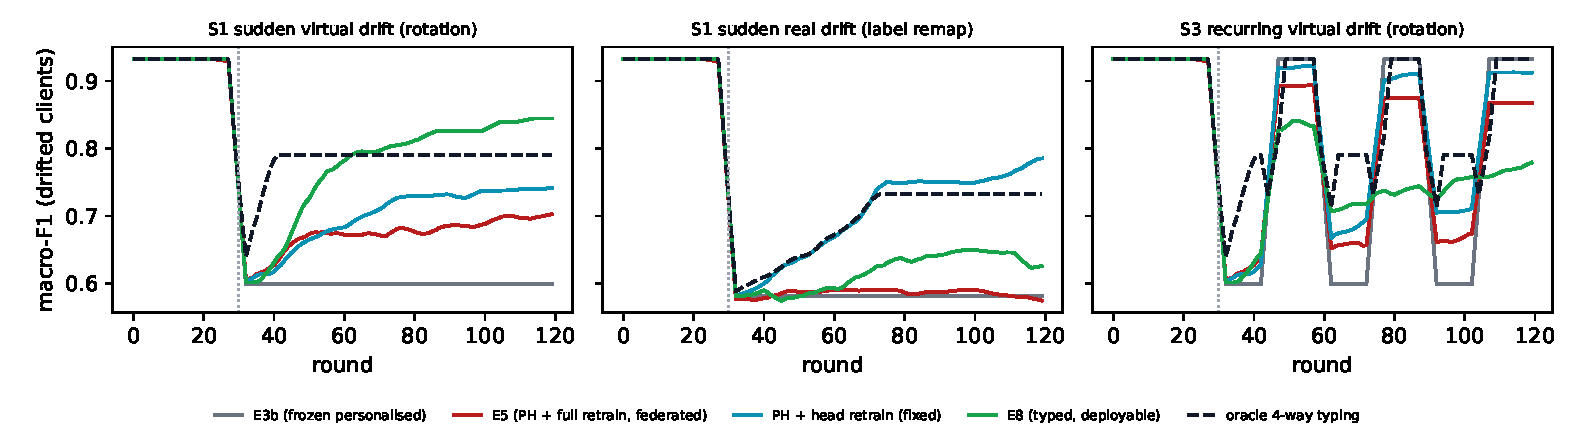
\includegraphics[width=\textwidth]{figs/recovery_curves.pdf}
\caption{Mean macro-F1 of the drifted clients over 10 evaluation seeds (5-round moving average). Dotted line: first onset (round 30). Rotation severity medium.}\label{fig:curves}
\end{figure*}

\begin{figure}[t]
\centering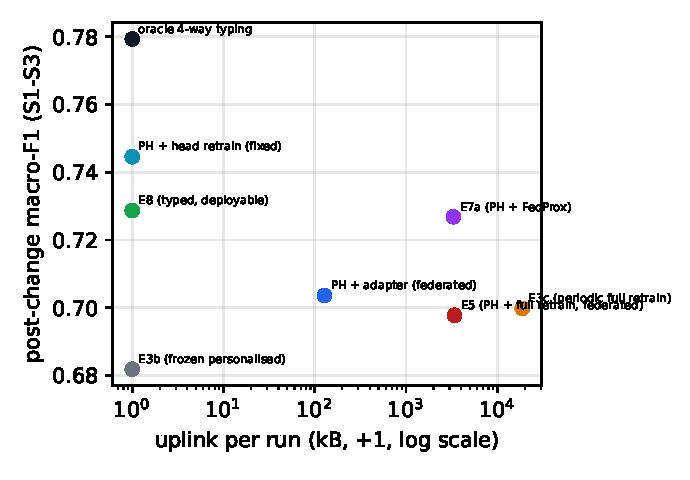
\includegraphics[width=0.85\columnwidth]{figs/pareto.pdf}
\caption{Post-change macro-F1 (mean over S1--S3 and seeds) against uplink per run.}\label{fig:pareto}
\end{figure}

\textbf{H1 (vs personalised FL): partly supported.} The deployable system improves on sudden drift ($+0.079$, Holm $p=0.023$) and the gradual-drift gain of $+0.080$ has a CI excluding zero but misses the corrected threshold ($p=0.078$). On recurring drift it is significantly \emph{worse} than the frozen model ($-0.050$): its F1 stays below the frozen model between drift episodes (Fig.~\ref{fig:curves}, right); we have not isolated the cause, and the likely one is a response (a kept recalibration, or head retraining) that is wrong once the drift has ended, since the deployable system has no revert step. \textbf{H2, H3:} no significant gain over periodic retraining or the FedProx variant on S1 and S2, and a significant loss against E7a on S3. \textbf{H5 (typed beats fixed): not supported.} The deployable typed system ties with always retraining the head on S1 and S2 ($+0.004$, $-0.016$) and is worse on S3 ($-0.055$); head retraining is a strong fixed response on this benchmark (averaged over virtual and real variants), and the typed system pays for mode-classification errors and the five-round typing delay (E8 vs the same system with the true mode: $-0.027$ S1, $-0.053$ S2, $-0.023$ S3).

\textbf{H4 (adapter vs full retraining): supported.} The federated adapter is non-inferior to full-model retraining E5 (E5 minus adapter: $-0.005$ [$-0.015$, $+0.005$] S1; $-0.002$ [$-0.013$, $+0.008$] S2; $-0.011$ [$-0.022$, $-0.000$] S3, all upper bounds below $+0.010$) with $96\%$ less uplink (127 vs 3387\,kB per S1 run). We stress that the responses that help most (input alignment, head retraining) are local and use no uplink at all, so the bandwidth saving of E8 over federated retraining is not attributable to adapter-style aggregation.

\subsection{What typing is worth}
With oracle labels, 4-way typing outperforms 2-way (virtual/real) typing by $+0.045$ on gradual, $+0.066$ on recurring and $+0.052$ on feature-level drift, and ties on sudden drift ($+0.000$), because tracking alignment, revert-and-restore of a cached fit, and sensor-restricted alignment need the finer type. This is an upper bound: classifying the 4-way type from \emph{detected} alarms was weak, so the benefit is not realised by the deployable system, and no confirmatory claim is made for it.

\section{Discussion and Limitations}\label{sec:disc}
\textbf{Detection is the bottleneck.} With an oracle trigger input alignment recovers $12$--$16$ points on virtual drift (tuning seeds); with the detector this is largely lost. Recall within 20 rounds stays at about $0.42$ for the best detector even with longer streams. \textbf{Full-model federated retraining did not help:} E3c, E4 and E5 improve on the frozen model by $0.02$--$0.03$ on S1 at 2.3--18.7\,MB of uplink, whereas local responses do as well or better at no cost. \textbf{Limitations.} A single dataset (PAMAP2, 8 clients, 12 classes) and injected rather than natural drift; the temporal split we examined mostly reflects bout-edge effects, not drift. Severity levels are ordinal within a transform and were calibrated once on a tuning seed. Alignment assumes immediate labels and a clean per-class reference on the client. The label budget (ablations on delayed labels, 1\%/5\%/20\%) and a recurring-drift memory for the deployable system were not evaluated; clustering and privacy mechanisms were not implemented, so we claim data locality only, not formal privacy. S0 streaming runs and the severity sweep were not run. Baselines are our re-implementations and E8's variance across seeds (std 0.05--0.08) is higher than the baselines' (about 0.02).

\section{Conclusion}
A client-side pipeline of error-stream detection, mode typing and local, label-conditioned recalibration recovers accuracy after sudden drift without uplink, and a federated adapter replaces full-model retraining at 4\% of the payload. The expected advantage of typing the response was not confirmed in deployable form: a fixed head-retraining response does as well on sudden and gradual drift, and the typed system loses on recurring drift. The oracle experiments indicate that better early detection and a memory for recurring drift are the next steps, which we leave as future work and do not claim here.

\bibliographystyle{IEEEtran}
\bibliography{refs}
\end{document}
